% Likelihood x impact of the residual risks (security-assessment, risk register). Cells list risk ids.
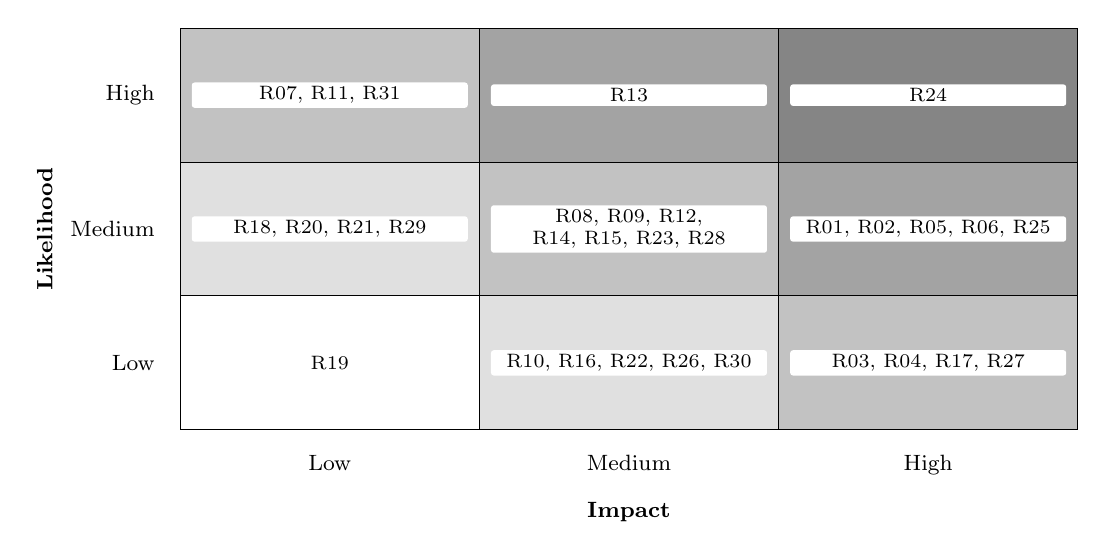
\begin{tikzpicture}[x=1mm,y=1mm]
  \def\cw{38}\def\ch{17}
  \foreach \i/\l in {0/Low,1/Medium,2/High} {
    \node[font=\footnotesize,anchor=east] at (-2,\i*\ch+\ch/2) {\l};
    \node[font=\footnotesize,anchor=north] at (\i*\cw+\cw/2,-2) {\l};
  }
  \node[font=\footnotesize\bfseries,rotate=90,anchor=south] at (-15,1.5*\ch) {Likelihood};
  \node[font=\footnotesize\bfseries,anchor=north] at (1.5*\cw,-8) {Impact};
  \foreach \x in {0,1,2} \foreach \y in {0,1,2} {
    \pgfmathsetmacro{\shade}{(\x+\y)*12}
    \fill[black!\shade!white] (\x*\cw,\y*\ch) rectangle ++(\cw,\ch);
    \draw (\x*\cw,\y*\ch) rectangle ++(\cw,\ch);
  }
  % cell contents: column = impact, row = likelihood
  \tikzset{cell/.style={font=\scriptsize,align=center,text width=34mm,fill=white,inner sep=1.5pt,rounded corners=1pt}}
  \node[cell] at (0.5*\cw,2.5*\ch) {R07, R11, R31};
  \node[cell] at (1.5*\cw,2.5*\ch) {R13};
  \node[cell] at (2.5*\cw,2.5*\ch) {R24};
  \node[cell] at (0.5*\cw,1.5*\ch) {R18, R20, R21, R29};
  \node[cell] at (1.5*\cw,1.5*\ch) {R08, R09, R12, R14, R15, R23, R28};
  \node[cell] at (2.5*\cw,1.5*\ch) {R01, R02, R05, R06, R25};
  \node[cell] at (0.5*\cw,0.5*\ch) {R19};
  \node[cell] at (1.5*\cw,0.5*\ch) {R10, R16, R22, R26, R30};
  \node[cell] at (2.5*\cw,0.5*\ch) {R03, R04, R17, R27};
\end{tikzpicture}
